\documentclass{acm_proc_article-sp}
\usepackage{tikz}
\usetikzlibrary{plotmarks}
\begin{document}
\title{Algorithm and Data Structure Coursework: \\PCA Features for
R-tree Based Similar Image Search}
\subtitle{}
%
\numberofauthors{2} %  in this sample file, there are a *total*
% of EIGHT authors. SIX appear on the 'first-page' (for formatting
% reasons) and the remaining two appear in the \additionalauthors section.
%
\author{
% You can go ahead and credit any number of authors here,
% e.g. one 'row of three' or two rows (consisting of one row of three
% and a second row of one, two or three).
%
% The command \alignauthor (no curly braces needed) should
% precede each author name, affiliation/snail-mail address and
% e-mail address. Additionally, tag each line of
% affiliation/address with \affaddr, and tag the
% e-mail address with \email.
%
\alignauthor
Qiwei Feng\\
       \affaddr{2011011250, IIIS-10}\\
       \affaddr{Tsinghua University}\\
       \email{gdfqw93@163.com}
\alignauthor
Pufan He\\
       \affaddr{2011011307, IIIS-10}\\
       \affaddr{Tsinghua University}\\
       \email{hpfdf@126.com}
}
\date{26 May 2015}

\maketitle
\begin{abstract}
This paper provides a sample of a \LaTeX\ document.
\end{abstract}

\keywords{R-Tree, Similar Image, PCA, K-Means}

\section{Introduction}

Github address: \texttt{https://github.com/caiwaifung/lastcourse}.

\subsection{Image Search}

\subsection{Data Structures}

\subsection{Low Level Features}

\subsection{PCA}

\subsection{K-Means}

\section{Data}

\section{Feature Finding}

TODO: list feature here (PCA, KMeans, Composite).

\section{R-Tree}
We use the ``rtree alternative package'' implementation of R-tree.
The wrapper \texttt{src/a.cpp} calls methods of provided R-tree class.
Run \texttt{python src/run.py} to compile and run the program.

\section{Experiments}

\subsection{Node Access Numbers}
Table \ref{table:accessnum} lists the node access number in different cases.
\begin{table} \centering 
    \caption{Node Access Numbers}
    \label{table:accessnum}
\begin{tabular}{|p{2.1cm}|c|c|c|c|c|}
    \hline
    Method and Feature Num & 1000 & 2000 & 3000 & 4000 & 5000 \\ \hline
    Color Moment HSV 9 & 46.11 & 67.69 & 88.69 & 98.24 & 117.0 \\ \hline
    PCA 4 & 37.18 & 53.31 & 71.37 & 76.72 & 81.83 \\ \hline
    PCA 8 & 68.42 & 107.7 & 145.8 & 176.1 & 208.4 \\ \hline
    PCA 12 & 77.95 & 129.9 & 174.5 & 217.8 & 252.6 \\ \hline
    PCA 16 & 82.46 & 135.4 & 190.2 & 236.2 & 280.0 \\ \hline
    PCA 20 & 81.55 & 137.8 & 196.4 & 253.7 & 302.8 \\ \hline
    PCA 24 & 83.11 & 135.7 & 192.8 & 248.0 & 297.4 \\ \hline
    PCA 30 & 123.8 & 207.4 & 281.4 & 351.7 & 416.4 \\ \hline
    KMeans 4 & 16.01 & 19.76 & 22.24 & 23.53 & 24.71 \\ \hline
    KMeans 8 & 17.49 & 21.83 & 24.44 & 25.88 & 26.66 \\ \hline
    KMeans 12 & 20.90 & 25.76 & 30.96 & 34.85 & 37.43 \\ \hline
    KMeans 16 & 22.22 & 28.40 & 33.89 & 37.25 & 38.14 \\ \hline
    KMeans 20 & 25.25 & 35.26 & 39.25 & 39.67 & 44.48 \\ \hline
    KMeans 24 & 20.68 & 27.81 & 30.20 & 33.46 & 34.79 \\ \hline
    Composite 25 & 80.01 & 136.8 & 202.4 & 254.9 & 305.4 \\ \hline
\end{tabular} \end{table}


The following graph shows the relationship between node access number
    and feature number.

\begin{center}
    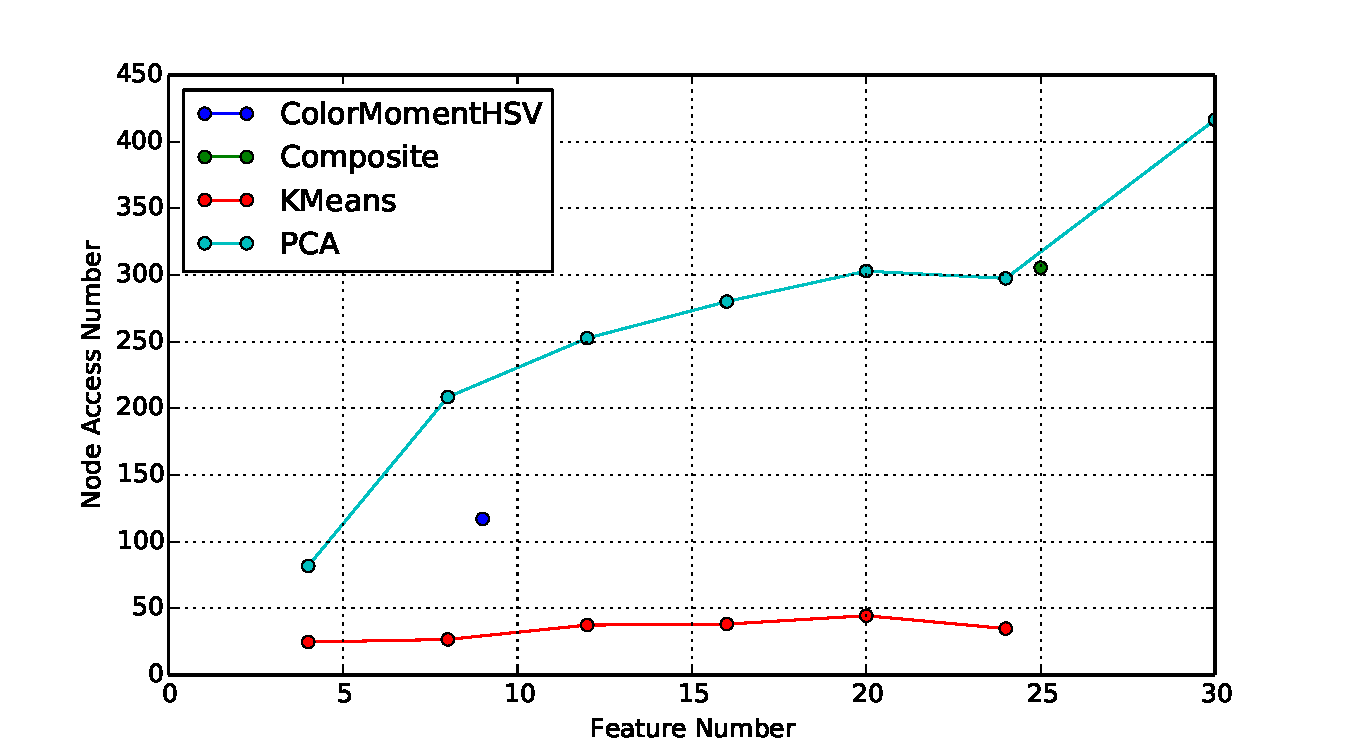
\includegraphics[width=0.4\textwidth]{data/accessnum.pdf}
\end{center}

\subsection{Performance}
Table \ref{table:correctness} lists the correctness for different feature.
There are 613 queries in total, and the database varies from 1000 images
    to 5000 images.
\begin{table} \centering 
    \caption{Correctness of Different Feature}
    \label{table:correctness}
\begin{tabular}{|p{2.1cm}|c|c|c|c|c|}
    \hline
    Method and Feature Num & 1000 & 2000 & 3000 & 4000 & 5000 \\ \hline
    Color Moment HSV 9 & 153 & 174 & 178 & 190 & 195 \\ \hline
    PCA 4 & 116 & 130 & 133 & 141 & 151 \\ \hline
    PCA 8 & 158 & 170 & 172 & 176 & 183 \\ \hline
    PCA 12 & 181 & 190 & 199 & 205 & 208 \\ \hline
    PCA 16 & 181 & 198 & 205 & 206 & 217 \\ \hline
    PCA 20 & 185 & 200 & 207 & 213 & 225 \\ \hline
    PCA 24 & 180 & 194 & 201 & 212 & 221 \\ \hline
    PCA 30 & 177 & 198 & 205 & 203 & 217 \\ \hline
    KMeans 4 & 126 & 132 & 147 & 148 & 147 \\ \hline
    KMeans 8 & 124 & 155 & 154 & 155 & 161 \\ \hline
    KMeans 12 & 132 & 154 & 158 & 154 & 158 \\ \hline
    KMeans 16 & 133 & 154 & 165 & 167 & 173 \\ \hline
    KMeans 20 & 132 & 160 & 157 & 159 & 164 \\ \hline
    KMeans 24 & 121 & 161 & 153 & 167 & 178 \\ \hline
    Composite 25 & 201 & 219 & 230 & 235 & 240 \\ \hline
\end{tabular} \end{table}

TODO: blahblah

\section{Conclusion}


\bibliographystyle{abbrv}
\bibliography{sigproc} 

\balancecolumns

\end{document}
